\documentclass[]{article}

\usepackage[utf8]{inputenc}
\usepackage[english,serbian]{babel}
\usepackage[margin=0.7in]{geometry}
\usepackage{url}
\usepackage{float}
\usepackage[graphicx]{realboxes}
\usepackage{listings}
\usepackage{textcomp}
\usepackage{xcolor}
\usepackage{titlesec}
\usepackage{adjustbox}
\lstset {
    language=HTML,
    frame=none,
    %xleftmargin=-.25in,
    %xrightmargin=.25in
    framesep=10pt,
    tabsize=4,
    showstringspaces=false,
    upquote=true,
    commentstyle=\color{black},
    keywordstyle=\color{black},
    stringstyle=\color{black},
    basicstyle=\small\ttfamily,
    emph={int,char,double,float,unsigned,void,bool},
    emphstyle={\color{black}},
    escapechar=\&,
    classoffset=1,
    morekeywords={>,<,.,;,,,-,!,=,~},
    keywordstyle=\color{black},
    classoffset=0,
    breaklines=true
}
\pagenumbering{gobble}

\titlespacing\title{left spacing}{before spacing}{after spacing}[right]

\title{Ra\v{c}unarske mre\v{z}e 4R, Ispit - Jan 1}
\date{11.01.2020.}

\begin{document}

\makeatletter
\begin{center}

{\fontsize{12pt}{14pt}\selectfont\bfseries\@title\par}
\@date

Pro\v{c}itati sve zadatke \textbf{pa\v{z}ljivo} pre rada - sve \v{s}to nije navedeno ne mora da se implementira! 

Vreme za rad: \textbf{2.5h}. Sre\'{c}no!
\end{center}
\makeatother


\begin{enumerate}
  \item Sockets \textbf{(16p)}
  \begin{itemize}
    \item Napraviti Java aplikaciju koja ima ulogu UDP servera. Slu\v{s}ati na portu 12345 i primiti datagrame od klijenata koriste\'c{}i \texttt{DatagramPacket} klasu. Sadr\v{z}aj svakog datagrama primljenog od klijenta je velicine \texttt{4B}. Ispisati tekst \texttt{Stigao datagram!} kad god server primi validan datagram od nekog klijenta. \hfill (3p)
    \item Napraviti Java aplikaciju koja ima ulogu UDP klijenta. Poslati UDP datagram lokalnom serveru na portu 12345 koriste\'c{}i \texttt{DatagramPacket} klasu. Sadr\v{z}aj datagrama je jedan pozitivan ceo broj veli\v{c}ine \texttt{4B} koji se unosi sa standardnog ulaza. \hfill (3p)
    \item Inicijalno, klijent \v{s}alje serveru datagram sa sadr\v{z}ajem koji predstavlja prirodni broj $n$ (ne ve\'c{}i od $80$). Nakon primanja datagrama, server klijentu \v{s}alje prvih $n$ Fibona\v{c}ijevih brojeva \footnote{Fibona\v{c}ijevi brojevi se ra\v{c}unaju po formuli: $F_0 = 0$, $F_1 = 1$, $F_n = F_{n-1} + F_{n-2}$ za $n > 1$}, po jedan u svakom datagramu. Svaki poslati broj je veli\v{c}ine \texttt{8B}. \hfill (4p)
    \item Primiti datagrame na klijentskoj strani, i za svaki primljeni datagram ispisati primljeni broj na standardni izlaz. \hfill (2p)
    \item Ke\v{s}irati Fibona\v{c}ijeve brojeve na serverskoj strani (ne ra\v{c}unati ih iznova za svakog klijenta). \hfill (2p)
    \item Postarati se da su svi resursi ispravno zatvoreni u slu\v{c}aju izuzetka. \hfill (1p)
  \end{itemize}

  \item Swing \textbf{(14p)}
  Napraviti Java Swing aplikaciju koja ima ulogu jednostavnog HTML editora. Izgled aplikacije je dat na slici ispod a HTML test primeri na slede\'c{}oj strani.
  \begin{itemize}
    \item Ispo\v{s}tovati izgled aplikacije (ne me\v{s}ati redosled komponenti i postarati se da su odnosi u veli\v{c}ini kao na slici). \hfill (2p)
    \item Napraviti prozor i u njega dodati skrolabilnu komponentu za prikaz HTML prezentacije. \hfill (2p)
    \item Omogu\'c{}iti da se prozor mo\v{z}e pro\v{s}iriti i smanjiti a da se raspored i razmera komponenti ne promeni. \hfill (2p)
    \item Dodati komponentu za unos URL-a koji vodi do HTML prezentacije (testirati na lokalnom fajl-sistemu koriste\'c{}i URL sa FILE protokolom). Dodati dugme \texttt{Prika\v{z}i} koje prikazuje prezentaciju sa datog URL-a u komponenti za prikaz. Ako URL nije validan ili ne vodi do HTML fajla, ispisati odgovaraju\'c{}u poruku u komponenti za prikaz. \hfill (4p)
    \item Dodati dugme \texttt{Ocisti} \v{c}iji je efekat da iz HTML fajla ukloni sve HTML tagove. Rezultat se prikazuje u komponenti za prikaz. \hfill (4p)
  \end{itemize}

  \begin{figure}[H]
    \centering
    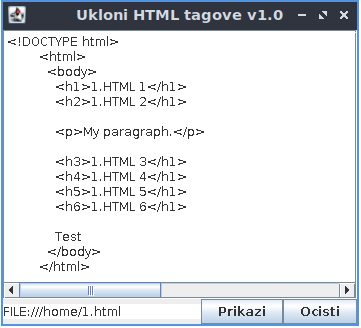
\includegraphics[scale=0.7]{fig1.PNG}
    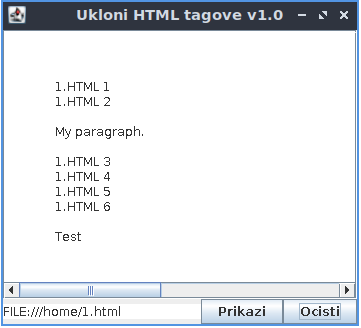
\includegraphics[scale=0.7]{fig2.PNG}
    \label{fig2}
    \caption{Izgled aplikacije pre i posle aktivacije dugmeta Ocisti}
  \end{figure}
\end{enumerate}


\newpage

HTML test fajlovi za zadatak 2:

\begin{itemize}
  \item 1.html
    \begin{lstlisting}
      <!DOCTYPE html>
        <html>
          <body>
            <h1>1.HTML 1</h1>
            <h2>1.HTML 2</h2>
            
            <p>My paragraph.</p>

            <h3>1.HTML 3</h3>
            <h4>1.HTML 4</h4>
            <h5>1.HTML 5</h5>
            <h6>1.HTML 6</h6>

            Test
          </body>
        </html>
    \end{lstlisting}
  \item 2.html
    \begin{lstlisting}
      <!DOCTYPE html>
        <html>
          <body>
            <h1>1.HTML 1</h1>
            <h2>1.HTML 2</h2>
            
            <p>My paragraph.</p>

            <h3>1.HTML 3</h3>

            Test

            <h1>1.HTML 1</h1>
          </body>
        </html>
    \end{lstlisting}
  \item 3.html
     \begin{lstlisting}
      <!DOCTYPE html>
        <html>
          <body>
            Test
            <h2>1.HTML 2</h2>
            <h4>1.HTML 4</h4>
            
            <p>My paragraph.</p>

            <h3>1.HTML 3</h3>

            Test

            <h1>1.HTML 1</h1>
          </body>
        </html>
    \end{lstlisting}
\end{itemize}


\end{document}
